\documentclass[12pt]{article}
\usepackage{amsmath}
\usepackage{amssymb}
\usepackage{graphicx}
%\usepackage{fancyhdr}
%\usepackage{geometry}
%\geometry{left=2.5cm,right=2.5cm,top=2.5cm,bottom=2.5cm}

%\pagestyle{fancy}

\date{}


%\cfoot{\thepage}
%\renewcommand{\headrulewidth}{0.5pt}
%\renewcommand{\footrulewidth}{0.0pt}
\begin{document}

The actual state space model of a linear process is given by
\begin{equation}\label{eq::state}
x_{t+1}=Ax_t+Bu_t
\end{equation}
\begin{equation}\label{eq:measurement}
y_t=Cx_t
\end{equation}
CVA is employed to identify the state space model. First, the data is stacked as follows
\begin{equation}
p_t=\begin{bmatrix}y_{t-1}^T & \ldots & y_{t-l}^T& u_{t-1}^T & \ldots & u_{t-l}^T\end{bmatrix}^T
\end{equation}
\begin{equation}
f_t=\begin{bmatrix}y_{t}^T & \ldots & y_{t+h}^T\end{bmatrix}^T
\end{equation}
Then, we perform singular value decomposition as follows
\begin{equation}
\Sigma_{pp}^{-1/2}\Sigma_{pf}\Sigma_{ff}^{-1/2}=UDV^T
\end{equation}
where $\Sigma_{pp}$ is the covariance of $p_t$, $\Sigma_{ff}$ is the covariance of $f_t$ and $\Sigma_{pf}$ is the covariance between $p_t$ and $f_t$. The canonical loading is computed by
\begin{equation}
J_k=U_k^T\Sigma_{pp}^{-1/2}
\end{equation}
where $U_k$ is the first $k$ columns of $U$. As such, the estimated state by CVA is given by
\begin{equation}
\hat{x}_t= J_kp_t
\end{equation}
The identified state space model is expressed as 
\begin{equation} \label{eq:identified}
\begin{bmatrix} \hat{A} & \hat{B}\\
                \hat{C} & \hat{D} \end{bmatrix} = \text{cov} (\begin{bmatrix} \hat{x}_{t+1}\\ 
                                                                              y_t \end{bmatrix}, \begin{bmatrix} \hat{x}_{t}\\ 
                                                                                                                u_t \end{bmatrix}) \text{cov}^{-1} (\begin{bmatrix} \hat{x}_{t}\\ 
                                                                                                                                                                    u_t \end{bmatrix},\begin{bmatrix} \hat{x}_{t}\\ u_t \end{bmatrix})
\end{equation}
Given the identified the state space model in Eq. \ref{eq:identified} and the actual state space model in Eqs. \ref{eq::state} and \ref{eq:measurement}, we are interested in finding a rotation matrix $R$ that relates the actual state $x_t$ and the identified state $\hat{x}_t$ as follows 
\begin{equation}
R^T\hat{x}_t=x_t
\end{equation}
where $R$ is a square matrix because it is assumed that the dimension of identified state is same as that of the actual state. The rotation matrix $R$ could be computed through least-squares estimation as follows
\begin{equation}\label{eq:rotation}
R=(\hat{\mathbf{X}}^T\hat{\mathbf{X}})^{-1}\hat{\mathbf{X}}^T\mathbf{X}
\end{equation}
where $\hat{\mathbf{X}}= \begin{bmatrix} \hat{x}_1 & \hat{x}_2 &\ldots &\hat{x}_N \end{bmatrix}^T$ and $\mathbf{X} = \begin{bmatrix} x_1 & x_2 & \ldots & x_N \end{bmatrix}^T$. Nevertheless, the actual state $x_t$ is not known. Note that Eqs. \ref{eq::state} and \ref{eq:measurement} are known, the actual state in Eq. \ref{eq:rotation} is replaced by the stated estimated by the Luenberger observer.
\begin{equation}
\tilde{x}_{t+1}=A\tilde{x}_t+L(y_t-C\tilde{x}_t)+Bu_t
\end{equation}
where $\tilde{x}_t$ is the state estimated by the Luenberger observer. Therefore, the rotation matrix $R$ relies on $A$, $B$, $C$ and $L$. In order to improve the accuracy in computing $R$, $\mathbf{X}$ is composed of the converged states estimated by the Luenberger observer.
Simulation results from a random linear system:
\begin{figure}[ht]
\begin{center}
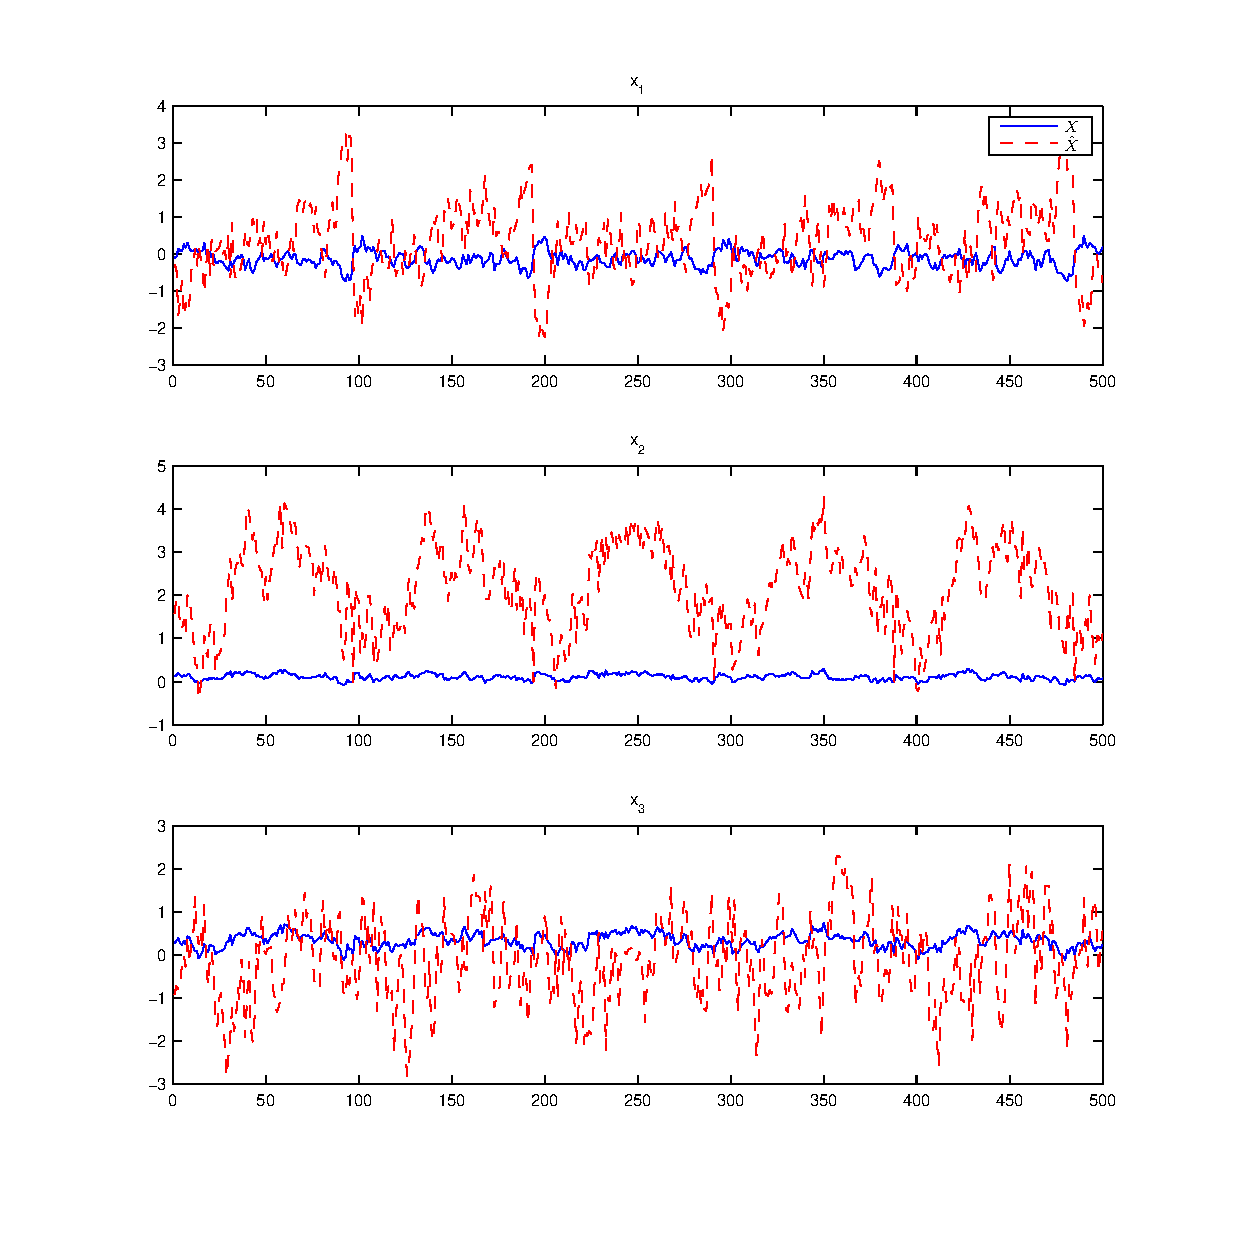
\includegraphics[width=4.5in]{statecompare1.eps}\\
\caption{$\mathbf{X}$ vs. $\hat{\mathbf{X}}$}
\label{fig:statecompare1}
\end{center}
\end{figure}

\begin{figure}[ht]
\begin{center}
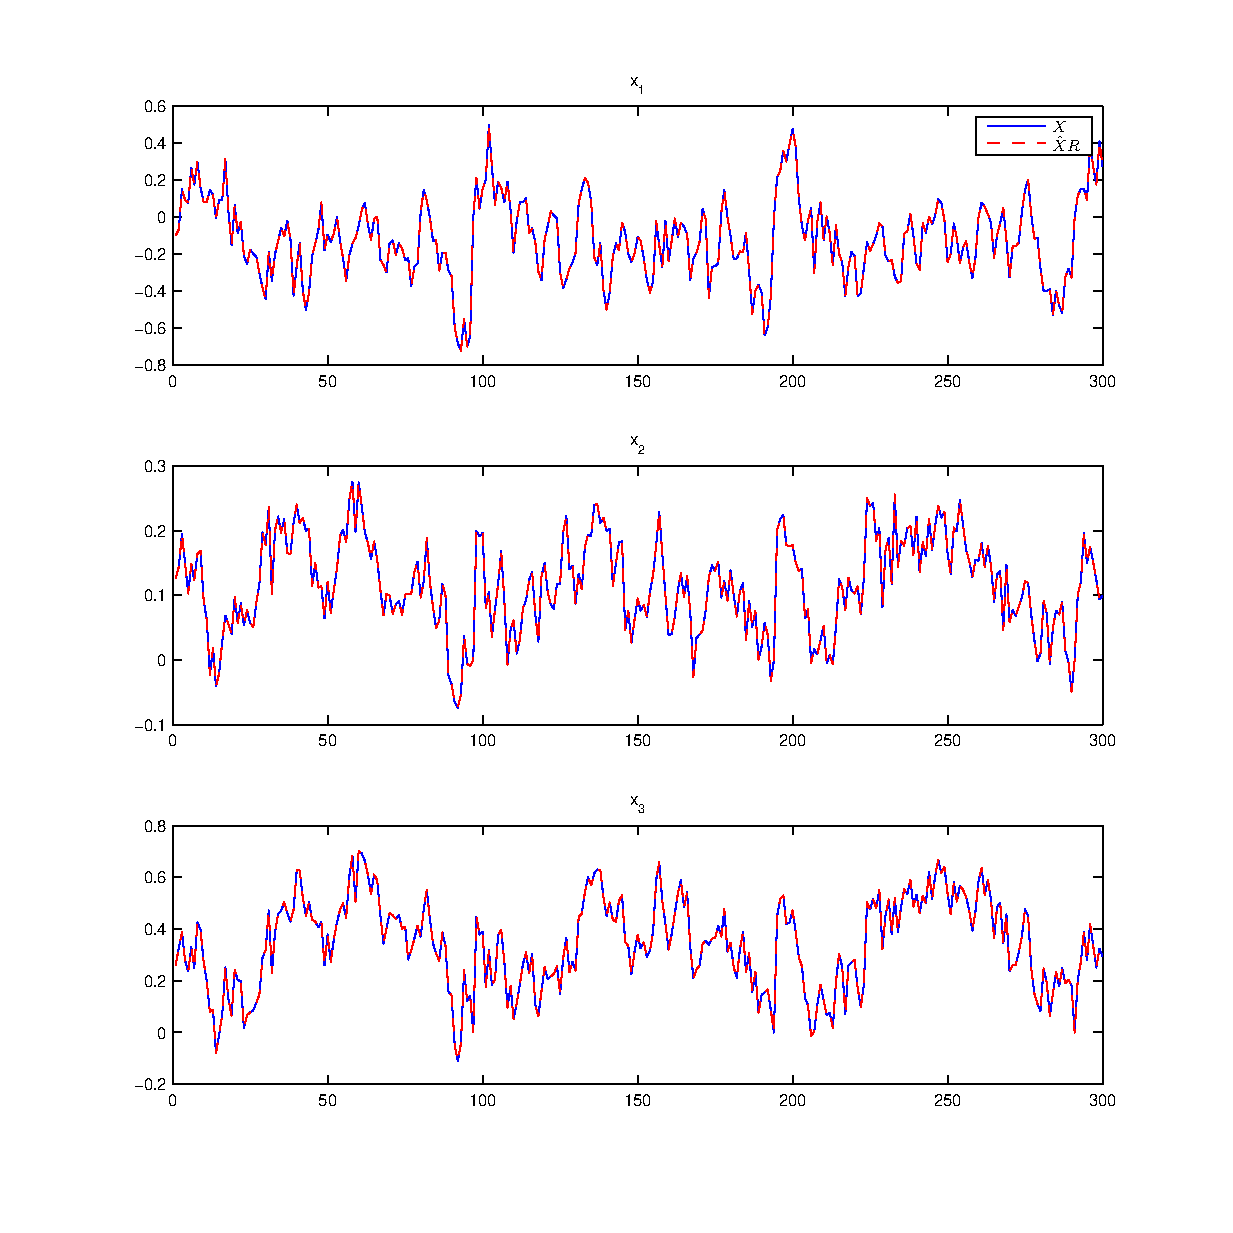
\includegraphics[width=4.5in]{statecompare2.eps}\\
\caption{$\mathbf{X}$ vs. $\hat{\mathbf{X}}R$}
\label{fig:statecompare2}
\end{center}
\end{figure}


































\end{document} 